\chapter{Results}
\label{chapter:results}

%5.0 Yleistä tuloksista
We first calculated internal and external validation metrics for 
the manually annotated subset of data to see how well our metrics 
revealed our defined ground truth clustering. Based on this we tried 
to evaluate the most suitable internal validation metric to be used 
with the complete data set. This validation metric would suggest us
the optimal number of clusters $k$ to be used in the clustering.
% Finally we inspect the resulting clustering
% and calculated internal validation metrics for it. 
% Finally we compare the clustering with the initial WOS subject 
% categories. [ei aikaa tähän]

%5.1 Manually annotated data  --> the chosen metrics
%5.3 Chosen number of clusters based on metrics (oikeasti tiedetään: 3)
%5.4 Klusterointi kolmeen
%5.5 Klustereiden havainnollistaminen
\section{Manually annotated data}
We evaluated our internal clustering validation metrics by 
creating a smaller subset of publications with manually
checked field of science (as described in Section 
\ref{sec:4clustering}). This subset consisted of 
$455$ publications from three different fields:
\emph{Computer science: Information systems}, $134$ publications,
\emph{Computer science: Artificial intelligence}, $127$ publications
and \emph{Clinical neurology}, $194$ publications.
The term frequency cut-off values $min_df=2$ (number of occurrences) 
and $max_df=0.5$ (portion of documents with the term) resulted
in $4455$ ignored terms and left the feature space of $3177$ terms. 
Terms that were filtered out as too frequent or too rare were for 
example: 
``haemoglobin\_a'', ``jacobian\_matrix'', 
``parthenogenetic'', ``chelation\_by\_saccharide\_molecules'', 
``leg\_blood\_supply'', ``computational\_fluid\_dynamics'', 
``pigment'', ``hdtv'', ``nicotinic\_receptor''. 
% Add line break due to random layout glitch
\linebreak
(Note: keywords were
combined with '\_' as described in Section \ref{sec:impl_preproc}.)
% \fixme{Then we calculated precision and recall for the data set.} 

The dimensionality of data was then reduced with LSA from $3177$
features (corresponding to the terms) to $800$ components which 
resulted $100\ \%$ of the explained variance of the data to be 
retained. The data was then agglomeratively clustered with Ward's 
method for number of cluster values $k=[2,12]$. 
The Figure \ref{fig:ch-silh01} shows the internal clustering 
validation results for these clusterings. 
\begin{figure}[ht]
  \begin{center}    
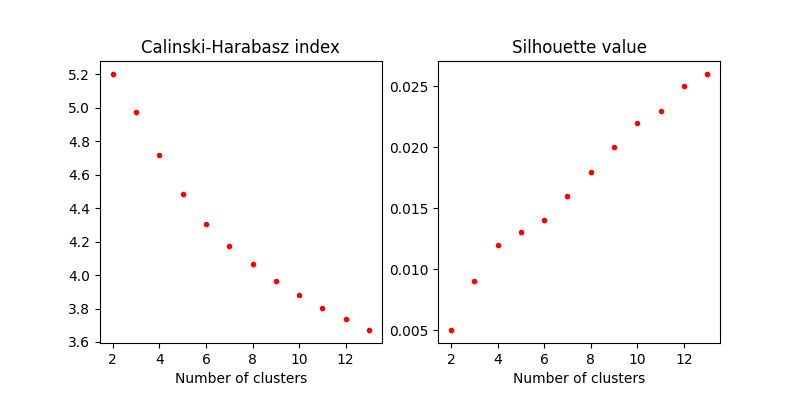
\includegraphics[width=11.5cm]{images/c-h-silh-index-plot-455-2_12-800-hierarchical.png}
    \caption{Calinski-Harabasz index and average silhouette values for the
    manually annotated set of 455 publications clustered with 
    hierarchical clustering, LSA with 800 components. The higher 
    value means more compact and better clustering in both 
    graphs.}
    \label{fig:ch-silh01}
    \end{center}
\end{figure}
We see that Calinski-Harabasz index reaches its maximum value 
with the number of clusters at two and that silhouette values 
increases with the number of clusters.
Neither of these indices suggests three clusters as the optimal 
clustering solution. So according these specific metrics the data 
doesn't support our initial idea of three ``natural'' clusters as
we meant it. We repeated the clustering in case of ambiguousness
in the algorithm but that didn't affect the clustering result.
Probably the low amount of samples compared to 
still quite high dimensional feature space affects here. We can 
conclude from the explained variance of $100\ \%$ that dimensionality
could have been reduced more. We also 
have to remember that Calinski-Harabasz index might suffer even 
from moderate noise \cite{liu_understanding_2010}.
% silhouette values (pros, cons...)

% reference: statistical significance samples relation dimension
% Perustelu ARI:n käyttämiseksi: eka katsottiin S ja C-H:lla josko
% toinen osuu k=3:een. Sitten katsottaan myös ARI:ll miten vahvasti
% k=3 erottuu muista k:n arvoista. Ei erotu juurikaan. Mitä tämä
% kertoo tai olisi kertonut?
% Jos olisi erottunut ja S tai C-H olisi erottunut: ok, yhteneväiset todistukset
% Jos olisi erottunut ja S tai C-H ei olisi: klusterointi on siellä mutta S ja C-H oleellisesti huonommat sen ilmaisemiseen (kenties klusterien rakenteen takia)
% Jos ei erotu ja S ja C-H erottaa: ei liene mahdollinen tilanne (?!) (ARI:n määritelmä?)
% Jos ei erotu ja S ja C-H ei erota: haluttu ja viereiset klusteroinnit yhtä epäselviä, data ei riitä/sovellu, tilanne nyt
We then use Adjusted Rand Index to check the quality of resulting 
clustering compared to ground truth. ARI tells us the similarity 
of the defined ground truth clustering and our resulting clustering. 
Figure \ref{fig:ari01} shows ARI values for different number of 
clusters $k=[2,12]$. Because ARI uses the ground truth cluster 
labels for the publications, it peaks at number of clusters at 
$3$. But we see that its value for $k=[4,6]$ is almost equally 
good. We interpret this to mean that each of these clusterings 
with $k=[3,6]$ have approximately equal amount of misclustered 
publications, so our clustering method can't actually find above 
others clustering for $k=3$ from this data.
\begin{figure}[htp]
  \begin{center}    
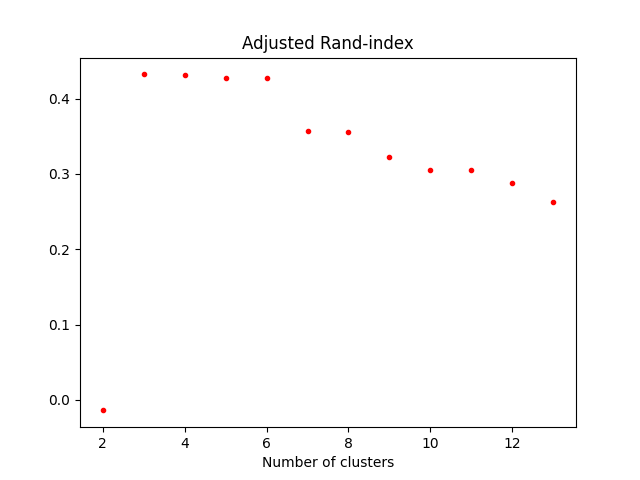
\includegraphics[width=7.5cm]{images/ari-plot-455-2_12-800-hierarchical.png}
    \caption{Hierarchical clustering. Adjusted Rand index for the
    manually annotated set of 455 publications clustered with
    hierarchical clustering, LSA with 800 components. The higher 
    value means more compact and better clustering. The index 
    gains its peak value with number of clusters at $3$.}
    \label{fig:ari01}
  \end{center}
\end{figure}

We inspected the resulting clustering for three clusters by 
looking at the most frequent terms of the publications in each 
cluster. Top 15 terms for each cluster are shown in the Table 
\ref{table:topterms_455_hier}. We can see that there is one cluster
with computer science related terms and two clusters with clinical
neurology related terms. So we can notice that our clustering method
didn't find the clusters we expected. This is also visible in 
adjusted Rand index values for the number of clusters $k=[3,6]$ almost 
equals (Figure \ref{fig:ari01}). For three clusters, part of the 
samples are incorrectly clustered, when compared against manual
labelling, and for clusterings with four to six clusters, the 
situation is obviously the same.

\begin{table}
\begin{tabular}{|p{2cm}|p{10.5cm}|} 
% Alignment of sells: l=left, c=center, r=right. 
% If you want wrapping lines, use p{width} exact cell widths.
% If you want vertical lines between columns, write | above between the letters
% Horizontal lines are generated with the \hline command:
\hline % The line on top of the table
\textbf{Cluster} & \textbf{Top terms} \\
\hline 
\textbf{1} & service image map system filter user som neural document mobile feature rule self-organizing logic query  \\
\hline
\hline 
\textbf{2} & dementia vascular vad trial subcortical cognitive alzheimer criterion impairment cause lesion stroke subtypes prevalence ad  \\
\hline
\hline 
\textbf{3} & stroke epilepsy pain treatment risk ad child seizure headache cognitive pd cortex parkinson cell apoe \\
\hline
\hline 
\end{tabular} % for really simple tables, you can just use tabular
% You can place the caption either below (like here) or above the table
\caption{Top terms for manually annotated dataset of 455 articles}
% Place the label just after the caption to make the link work
\label{table:topterms_455_hier}
\end{table} % table makes a floating object with a title 


For a comparison we also tried clustering manually annotated data
with K-means clustering. The idea was to see if this method would
give clearer clusters where the clustering that either silhouette values or 
Calinski-Harabasz index would recognize. Its similar
index values for number of clusters $k=[2,12]$ can be seen in 
figure \ref{fig:ch-silh02}. K-means wasn't able to significantly 
improve the clustering.

\begin{figure}[htp]
  \begin{center}    
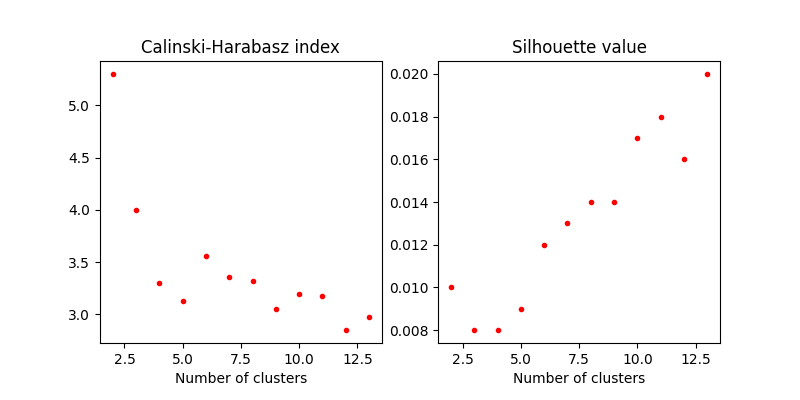
\includegraphics[width=11.5cm]{images/c-h-silh-index-plot-455-2_12-800-kmeans.png}
    \caption{Calinski-Harabasz index and average silhouette values for the
    manually annotated set of 455 publications clustered with 
    \emph{K-means clustering}, LSA with 800 components. The higher
    value means more compact and better clustering in both graphs.}
    \label{fig:ch-silh02}
  \end{center}
\end{figure}

We can see that both our internal validation methods indicate that
our clustering method doesn't find significant clusterings for
expected three clusters.
% From Table \ref{} we can see the Calinski-Harabasz index values.
As a result we also don't get strong support for using any of 
these two measures to decide the number of clusters for the actual 
one year data.
We cluster next the full data for years 2000-2001 to see if more 
data improves the clustering results.

%5.2 Metrics evaluation, also compare to precision and recall??
% \subsection{Precision and recall}
% With manually annotated dataset of 455 articles we compared 
% the results with three clusters which was assumed the correct 
% classification of the data set. We got recall $R = ???$ and 
% precision $P = ???$ which is
% a quite poor result. By looking at the top terms and random samples
% from each cluster we notice that two of the three clusters have 
% \emph{'Clinical neurology'} related items, see Tables
% \ref{table:topterms_455_hier} and \ref{table:articles_455_hier}.

% \begin{table}
\begin{tabular}{|p{2cm}|p{10.5cm}|} 
% Alignment of sells: l=left, c=center, r=right. 
% If you want wrapping lines, use p{width} exact cell widths.
% If you want vertical lines between columns, write | above between the letters
% Horizontal lines are generated with the \hline command:
\hline % The line on top of the table
\textbf{Cluster} & \textbf{Top terms} \\
\hline 
\textbf{1} & service image map system filter user som neural document mobile feature rule self-organizing logic query  \\
\hline
\hline 
\textbf{2} & dementia vascular vad trial subcortical cognitive alzheimer criterion impairment cause lesion stroke subtypes prevalence ad  \\
\hline
\hline 
\textbf{3} & stroke epilepsy pain treatment risk ad child seizure headache cognitive pd cortex parkinson cell apoe \\
\hline
\hline 
\end{tabular} % for really simple tables, you can just use tabular
% You can place the caption either below (like here) or above the table
\caption{Top terms for manually annotated dataset of 455 articles}
% Place the label just after the caption to make the link work
\label{table:topterms_455_hier}
\end{table} % table makes a floating object with a title 

% \begin{table}
\begin{tabular}{|c|p{6.5cm}|p{4.7cm}|} 
\hline % The line on top of the table
\textbf{ } & \textbf{Title} & \textbf{WoS category} \\ 
\hline 
\multirow{ 5}{*}{\textbf{1}} & Attacks against the WAP WTLS protocol & CS\_INFORMATION\_SYS \\
& Bringing knowing-when and knowing-what together: Periodically tuned categorizati & CS\_ARTIFICIAL\_INT  \\
& A digital television service architecture & CS\_INFORMATION\_SYS  \\ 
& A wavelet transform method for coding film-grain noise corrupted images & CS\_ARTIFICIAL\_INT  \\ 
& Accuracy of pedicle screw insertion with and without computer assistance: a rand & CLINICAL\_NEUROLOGY  \\
\hline
\hline 
\multirow{ 5}{*}{\textbf{2}} & Is subcortical vascular dementia a clinical entity for clinical drug trials? & CLINICAL\_NEUROLOGY \\
& Research criteria for subcortical vascular dementia in clinical trials & CLINICAL\_NEUROLOGY \\
& Subcortical vascular dementia as a specific target for clinical trials & CLINICAL\_NEUROLOGY \\ 
& Prognosis with dementia in Europe: A collaborative study of population-based coh & CLINICAL\_NEUROLOGY \\ 
& Comparison of different clinical criteria (DSM-III, ADDTC, ICD-10, NINDS-AIREN, & CLINICAL\_NEUROLOGY \\
\hline
\hline 
\multirow{ 5}{*}{\textbf{3}} & Interferon-alpha 2a effects on complement activation and regulation in MS patien & CLINICAL\_NEUROLOGY \\
& Architectural evolution - Nokia mobile phone case & CS\_INFORMATION\_SYS \\
& CASCADE: A European collaborative study on vascular determinants of brain lesion & PUBL\_ENVTL\_OCCUPA  \\ 
& Natural history of unruptured intracranial aneurysms: probability of and risk fa & CLINICAL\_NEUROLOGY \\ 
& An FDOPA PET study in patients with periodic limb movement disorder and restless & CLINICAL\_NEUROLOGY \\
\hline
\hline 
\end{tabular} % for really simple tables, you can just use tabular
\caption{Five random articles per cluster for manually annotated dataset of 455 articles}
\label{table:articles_455_hier}
\end{table} % table makes a floating object with a title


% \subsection{Other metrics}
% Different metrics to evaluate clustering include (from 
% scikit-learn) Adjusted Rand Index, Mutual Information scores 
% (NMI, AMI), homogenity, completness, V-measure, Fowlkes-Mallows 
% scores, Silhouette Coefficient, Calinski-Harabaz Index, (from 
% sources) 


%5.2 Finnish publications
\section{Finnish publications from years 2000-2001}
The analysis of full data set followed the same steps as for 
the manually annotated data except we couldn't calculate adjusted
Rand index because of the lacking ground truth.
% Vectorising
Vectorising the two years of data, $21155$ publications, with term 
frequency cut-off values $min_df=2$
(number of occurrences) and $max_df=0.1$ (portion of documents with
the term) and maximum number of terms $50000$ resulted $101333$ 
ignored terms and a feature space of $50000$ most frequent terms 
just below the $max_df=0.1$ threshold. 
% $\{2, 4, 6, 8, 10, 12, 14, 16, 18, 20, 26, 33, 40, 47, 54, 61, 
% 68, 75, 82, 89, 96, 103, 110, 117, 124, 131, 138, 145, 152, 159,
% 166, 173, 180, 187, 194, 201, 208, 215, 222, 229, 236, 243, 250,
% 251, 254, 257, 260\}$
This feature space was then reduced with LSA to $800$ component 
reduced space. In this dimensionality reduction 35 \% of the 
explained variance of the $50000$ term feature space data was retained.
The data was then clustered using Ward's method with selected 
values of number of clusters in the range of $k=[4,500]$ to find 
the optimal value for $k$.
The Calinski-Harabasz and average silhouette values for this range
are shown in Figure \ref{fig:ch-silh-2000-h}.
\begin{figure}[htp]
  \begin{center}    
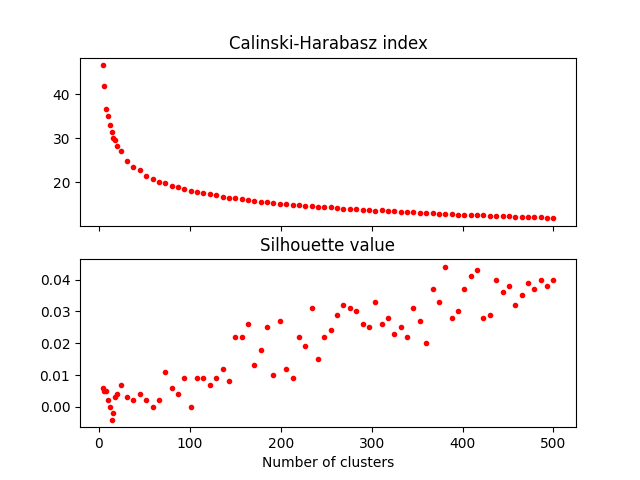
\includegraphics[width=10cm]{images/c-h-silh-index-plot-22000-4_500-800-hierarchical.png}
    \caption{Calinski-Harabasz index and average silhouette values 
    for Ward's clusterings the 2000-2001 Finnish publications data
    with number of clusters $4-500$. The higher value mean more 
    compact and better clustering in both graphs.}
    \label{fig:ch-silh-2000-h}
  \end{center}
\end{figure}
We can see that the index values follow the same pattern as with 
the manually annotated data. Again Calinski-Harabasz index 
suggests that optimal clustering is reached with very few clusters
while silhouette values tells us that clusterings improve with 
increasing number of clusters. Because these cluster validation 
measures are in conflict we chose a compromise value for the 
number of clusters, $188$, for further inspection. We chose this 
as a haphazard sample in the order of magnitude of current amount 
of WoS subject categories ($254$).
We wanted to validate by looking into clusters whether there would
be some meaningful clustering.
%or not, as suggested by the validation metrics.

% Silhouette plot
We first plotted the silhouette of this clustering in Figure 
\ref{fig:silh01}.
\begin{figure}[htp]
  \begin{center}    
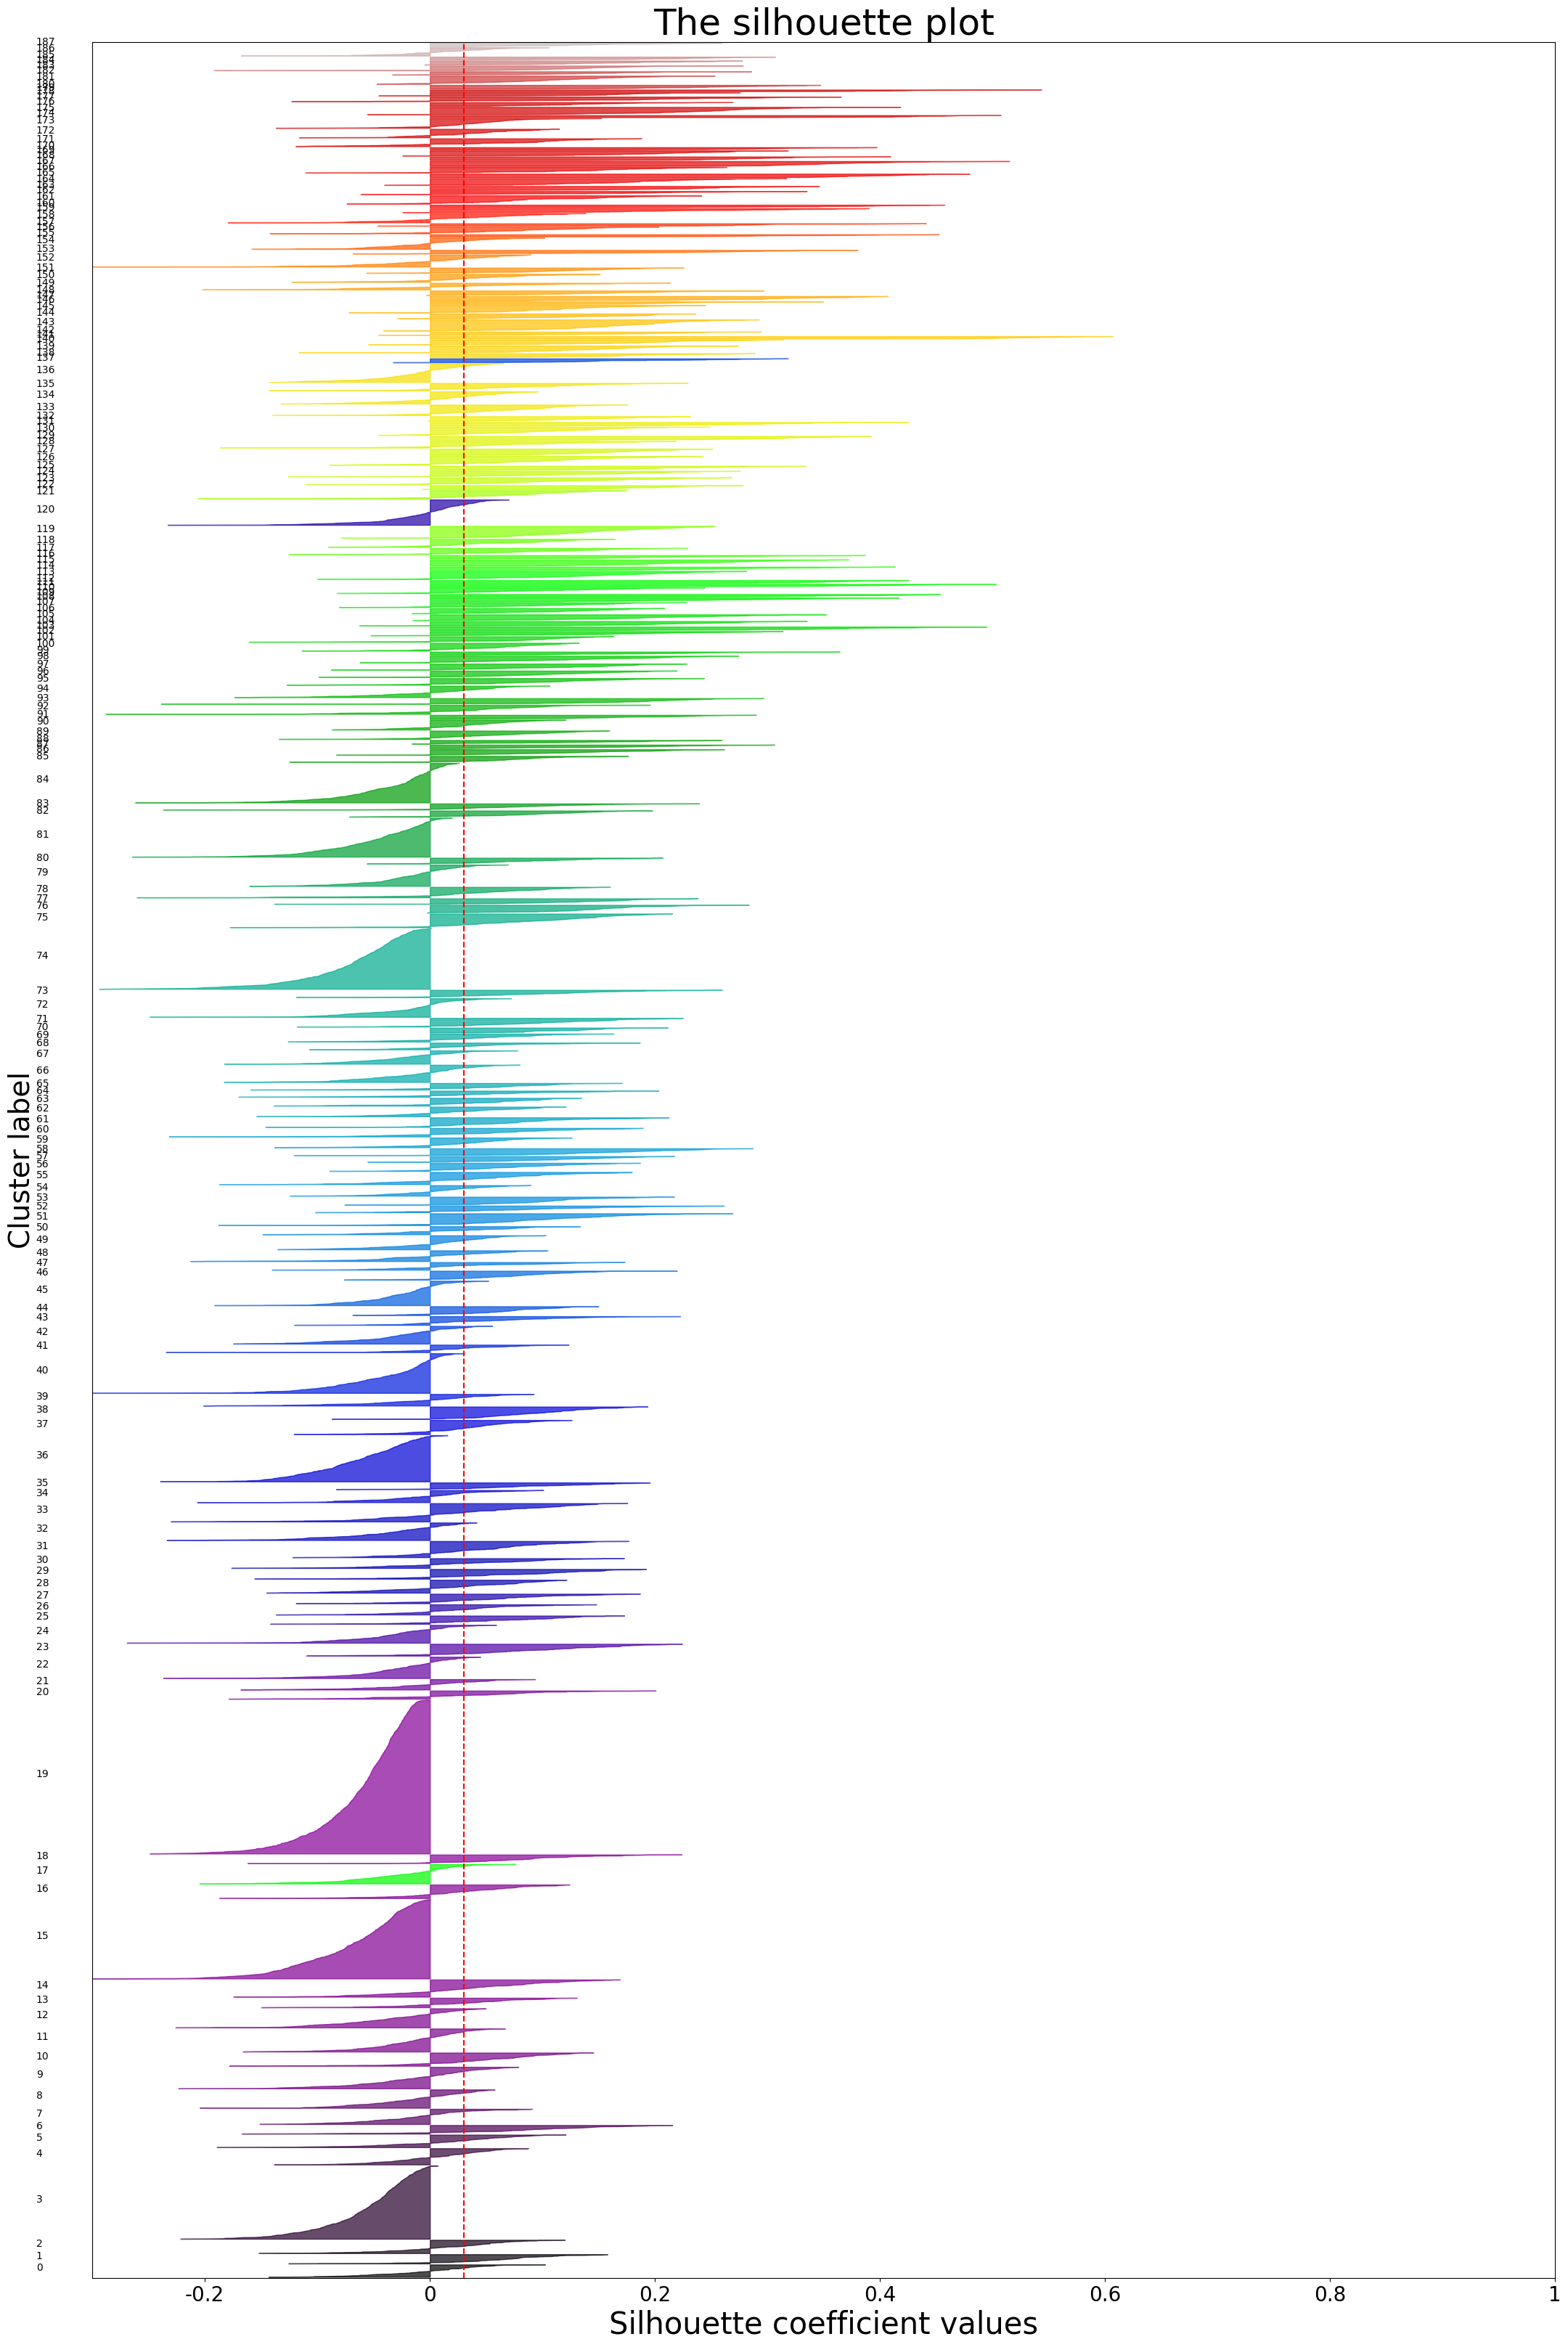
\includegraphics[width=13cm]{images/21155-188-800-hierarchical-silhouette.png}
    \caption{Silhouette values of 188 clusters. Repeating shapes
    are clusters consisting of stacked thin horizontal lines of 
    silhouette values of individual items. Colour indicates the 
    cluster. Contrasting coloured ones are the sample clusters.
%     A line more into positive axis direction indicates an item
%     better clustered. Value near zero means an item could almost
%     equally well be clustered in its nearest neighboring cluster.
%     Negative value means likely misclustered item.
%     Each thin horizontal line corresponds to a silhouette value of
%     an item. Lines are stacked to adjacent rows separated by gap 
%     corresponds to a cluster.
    Dashed line is the average over whole clustering.}
    \label{fig:silh01}
  \end{center}
\end{figure}
Colour indicates the cluster. Each cluster consists of stacked and 
infinitesimally thin horizontal lines. Each line corresponds a
silhouette value of a publication in its cluster. 
From the plot we see that some of the clusters are limited in size
and well clustered indicated by thinner horizontal silhouettes
extending further to the positive axis direction. There are also 
few very big clusters
of items poorly clustered among their neighbouring items indicated 
by broader silhouettes extending to the negative axis direction. Many clusters
have both components, resulting a silhouette resembling bow tie. 
Short lines as part of a silhouette indicate items that could 
almost equally well be clustered in their nearest neighbouring cluster.
As a result the average silhouette value of this clustering $0.030$,
(dashed line in the plot) is 
very low in absolute terms considering its index space [-1,1].

% Top terms inspection
By inspecting the top 15 terms of three random clusters sampled 
from $188$ in Table \ref{table:topterms-188-h-short},
\begin{table}[htp]
  \begin{center}
    \pgfplotstabletypeset[
    col sep=colon,
    verb string type,
    begin table=\begin{longtable},
    end table=\end{longtable},
    columns/cluster/.style={column name={Cluster}, column type={|l}},
    columns/top terms/.style={column name={Top terms}, column type={|p{115mm}|}},
    every even row/.style={before row={\rowcolor[gray]{0.9}}},
    every head row/.style={before row=\hline,after row=\hline},
    every head row/.append style={after row=\endhead},
    every last row/.style={after row=\hline}
]{../data/processed/topterms/12000-188-800-hierarchical-topterms-short.csv}



    \caption{Top terms for three random clusters from total 188}
    \label{table:topterms-188-h-short}    
 \end{center}
\end{table}
we note that at least these three clusters seem reasonable. The 
cluster 9 contains terms perhaps from some production technology
area, the cluster 19 seems to contain computer science related
terms and the cluster 31 medical research related terms.
% Publication title & WoS category inspection
To get little more concrete understanding of these clusters, we 
listed five random publication titles and their WoS subject 
categories in the Table \ref{table:articles-188-h-mini}. (See 
Appendices \ref{chapter:second-appendix} and 
\ref{chapter:appendix-articles} for top term and publication 
title lists for ten sample clusters respectively.)
% Pari sanaa julkaisuotsikoista ja WoS-luokituksista
We can now compare our first impression of these three clusters, 
given by top terms, to full publication titles and WoS subject 
categories inherited from the journal in which a publication was
published. The cluster 9 turns out to be a mixed cluster of quite
diverse publications including political science, psychology, 
ecology and forestry. The cluster 19 contains computer science 
related publications but also a publication related to music that 
could be an outlier. The sample publications of cluster 31 are all
related to medical sciences. 
\newpage
% JPL: data from: data/processed/12000-188-800-hierarchical-results.txt

\newcolumntype{g}{>{\columncolor{gray!20}}p{5.7cm}}
% \begin{longtable}{|p{0.9cm}|p{6.5cm}|p{5.0cm}|}
\begin{longtable}{|p{0.9cm}|g|g|}
\caption{Five random articles for three random clusters out of 188 clusters for the publications of year 2000}
\label{table:articles-188-h-mini}
\hline % The line on top of the table
\rowcolor{white}
  \textbf{Clust} & \textbf{Title} & \textbf{WoS category} \\
\hline
\hline
\rowcolor{white}
  \multirow{ 5}{*}{\textbf{9}} & Size of environmental grain and resource matching & ECOLOGY \\
& A note on Matthias Sutter & POLITICAL SCIENCE  \\
\rowcolor{white}
  & National outdoor recreation demand and supply in Finland: an assessment project & FORESTRY  \\
& Industrial ecology of the paper industry &   \\
\rowcolor{white}
  & Sex differences in quality of life among allogeneic BMT recipients & PSYCHOLOGY; SOCIAL SCIENCES BIOMEDICAL  \\
\hline

\multirow{ 5}{*}{\textbf{19}} & Neuron weight dynamics in the SOM and Self-Organized Criticality & COMPUTER SCIENCE ARTIFICIAL INTELLIGENCE; ENGINEERING ELECTRICAL ELECTRONIC \\
\rowcolor{white}
  & Indexing text with approximate q-grams & COMPUTER SCIENCE THEORY METHODS \\
& XML based text TV & COMPUTER SCIENCE INFORMATION SYSTEMS; ENGINEERING ELECTRICAL ELECTRONIC; TELECOMMUNICATIONS \\
\rowcolor{white}
  & Musical networks: Parallel distributed perception and performance. & PSYCHOLOGY EXPERIMENTAL; MUSIC \\
& PARNEU: general-purpose partial tree computer & COMPUTER SCIENCE HARDWARE ARCHITECTURE; COMPUTER SCIENCE THEORY METHODS; ENGINEERING ELECTRICAL ELECTRONIC \\
\hline

\rowcolor{white}
  \multirow{ 5}{*}{\textbf{31}} & Citalopram controls phobic symptoms in patients with panic disorder: randomized controlled trial & NEUROSCIENCES PSYCHIATRY PSYCHIATRY \\
& Long-term treatment of psoriasis with calcipotriol scalp solution and cream & DERMATOLOGY VENEREAL DISEASES \\
\rowcolor{white}
  & Docetaxel, a promising novel chemotherapeutic agent in advanced breast cancer & ONCOLOGY \\
& Silica xerogel as an implantable carrier for controlled drug delivery - evaluation of drug distribution and tissue effects after implantation & ENGINEERING BIOMEDICAL; MATERIALS SCIENCE BIOMATERIALS \\
\rowcolor{white}
  & A double-blind, randomized study to compare the efficacy and safety of terbinafine (Lamisil (R)) with fluconazole (Diflucan (R)) in the treatment of onychomycosis & DERMATOLOGY VENEREAL DISEASES \\
\hline
\end{longtable}


In Figure \ref{fig:silh01} these clusters are coloured with 
contrasting colours, green and blue. (Cluster numbering got mixed, 
so in the figure they have different positions.)
% alin vihreä klusteri == cluster 31
The lowest green cluster corresponds to the cluster 31. 
Regardeless of the consistent top terms and the sample of 
publication titles the cluster has its silhouette values in 
$[-0.2, 0.1]$ range and the negative part of the silhouette is 
slightly larger than positive. This tells us that the cluster 
isn't very coherent when half of its items seems to be 
misclustered. 
% toka sininen klusteri == cluster 9
The second blue cluster in the upper part of 
the plot corresponds to the cluster 9. It has similar silhouette 
shape with cluster 31 which is in line with the mixed sample of 
titles it contains. 
% ylin sininen klusteri == cluster 19
The blue top cluster corresponds to the cluster 19. Its values are
in the $[-0.05, 0.35]$ range which promises for a more meaningful 
cluster. This is in line with the top term list and the sample of 
titles.
We see even from this narrow glimpse that the clustering wasn't 
satisfactory. While the cluster 31 seemed consistent by top terms 
and the sample of its titles, the silhouette values tells otherwise.
Top terms and sample titles of clusters 9 and 19 are more in line
with their silhouette values. Generally these random samples show
that clustering like this can't substitute currently used 
classifications.



% A comparison to K-means clustering in the Figure 
% \ref{fig:ch-silh-full-h}...
%
% \begin{figure}[ht]
%   \begin{center}    
% 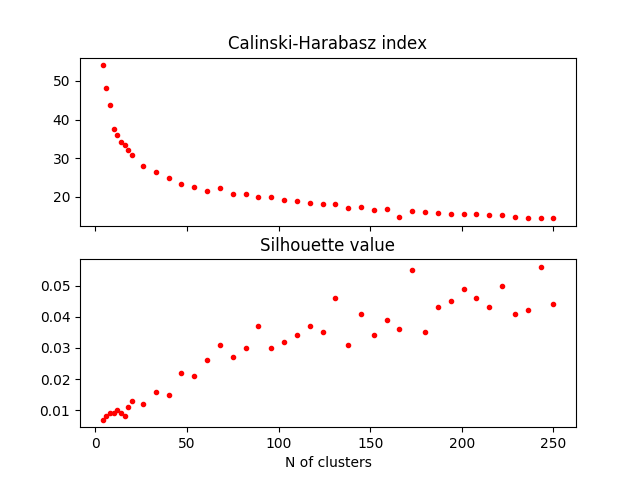
\includegraphics[width=10cm]{images/c-h-silh-index-plot-y2000-2_260-800-kmeans.png}
%   \caption{Calinski-Harabasz index and average silhoutte values of $10145$
%   items clustered with K-means clustering, LSA with 800 components. 
%   The higher value mean more compact and better clustering in both graphs.}
%     \label{fig:ch-silh-full-h}
%   \end{center}
% \end{figure}
